\chapter{Results}
\label{chap:results}

This chapter reports the complete QASPER test retrieval evaluation before turning to supplementary mechanism and generation analyses. The central comparison is ControllerV3 against BM25 top-7, which has almost the same average estimated evidence cost. Results are reported at overlap threshold 0.5 unless stated otherwise.

\section{Fixed-depth quality--cost frontier}

\Cref{tab:retrieval-main} shows a clear progression as the fixed BM25 budget increases. Evidence Recall rises from 0.2187 at top-1 to 0.9538 at top-20, while average estimated tokens rise from 224 to 4,014. Question Hit Rate similarly rises from 0.3824 to 0.9867. The additional coverage is therefore purchased with a much larger evidence context.

\begin{table}[tb]
\centering
\caption{Retrieval quality and cost on the complete QASPER test split at overlap threshold 0.5. Evidence metrics use 1,352 questions with annotated evidence; cost uses all 1,451 questions.}
\label{tab:retrieval-main}
\small
\begin{tabular}{@{}lrrrrr@{}}
\toprule
Method & Recall & Hit rate & Avg. units & Est. tokens & Recall/1k \\
\midrule
BM25 top-1 & 0.2187 & 0.3824 & 1.00 & 224 & 0.9763 \\
BM25 top-3 & 0.4592 & 0.6657 & 3.00 & 694 & 0.6617 \\
BM25 top-5 & 0.6149 & 0.8003 & 5.00 & 1,171 & 0.5251 \\
BM25 top-7 & 0.7059 & 0.8624 & 7.00 & 1,629 & 0.4333 \\
BM25 top-8 & 0.7442 & 0.8876 & 8.00 & 1,864 & 0.3992 \\
BM25 top-10 & 0.8084 & 0.9127 & 9.99 & 2,305 & 0.3507 \\
BM25 top-20 & 0.9538 & 0.9867 & 19.27 & 4,014 & 0.2376 \\
\midrule
ControllerV3 & 0.7099 & 0.8706 & 7.76 & 1,638 & 0.4334 \\
ControllerV3 no section & 0.6879 & 0.8558 & 7.27 & 1,534 & 0.4484 \\
\bottomrule
\end{tabular}
\end{table}

Recall per 1,000 estimated tokens declines as fixed $k$ grows. This pattern is expected for a ranked list: high-value lexical matches tend to occur early, while later units add fewer newly covered gold spans. The ratio should not be optimised in isolation. Top-1 has the highest ratio but fails to hit annotated evidence for nearly 62\% of eligible questions. The practical frontier therefore requires a minimum acceptable quality as well as a cost preference.

\begin{figure}[tb]
\centering
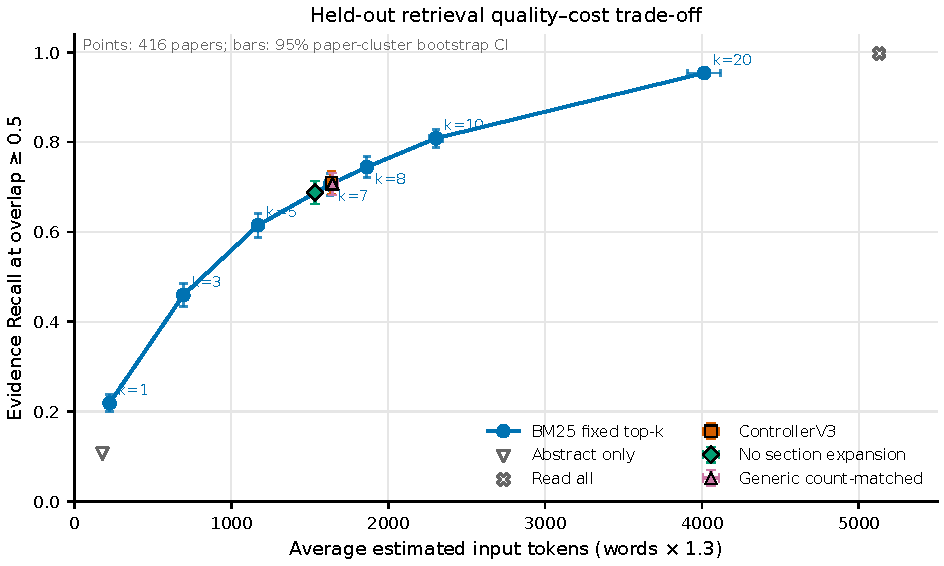
\includegraphics[width=0.92\textwidth]{figures/fig_retrieval_quality_cost.pdf}
\caption{Evidence Recall and Question Hit Rate against average estimated evidence tokens on the complete QASPER test split.}
\label{fig:quality-cost}
\end{figure}

\section{ControllerV3 against fixed budgets}

ControllerV3 obtains 0.7099 Evidence Recall and 0.8706 Question Hit Rate at an average cost of 1,638 estimated tokens. It sits between BM25 top-5 and top-8 on both quality and cost, and is almost cost-matched to top-7. Relative to top-5, the controller reads about 467 more estimated tokens and improves recall by 0.0950 (95\% paired interval [0.0809, 0.1087]) and hit rate by 0.0703 [0.0533, 0.0876]. Relative to top-10, it uses about 667 fewer estimated tokens, with recall lower by 0.0985 and hit rate lower by 0.0422. These comparisons describe a tunable trade-off rather than domination of the fixed baselines.

The cost-matched comparison is more revealing. ControllerV3 exceeds top-7 by 0.0040 recall, 0.0081 hit rate, and 8.1 estimated tokens. The 95\% paired intervals are $[-0.0118,0.0184]$ for recall, $[-0.0044,0.0210]$ for hit rate, and $[-13.4,29.4]$ for estimated tokens. None shows a clear sampled difference. The correct conclusion is that the two methods have close point estimates at similar average cost; the experiment neither establishes a controller advantage nor proves equivalence.

\begin{figure}[tb]
\centering
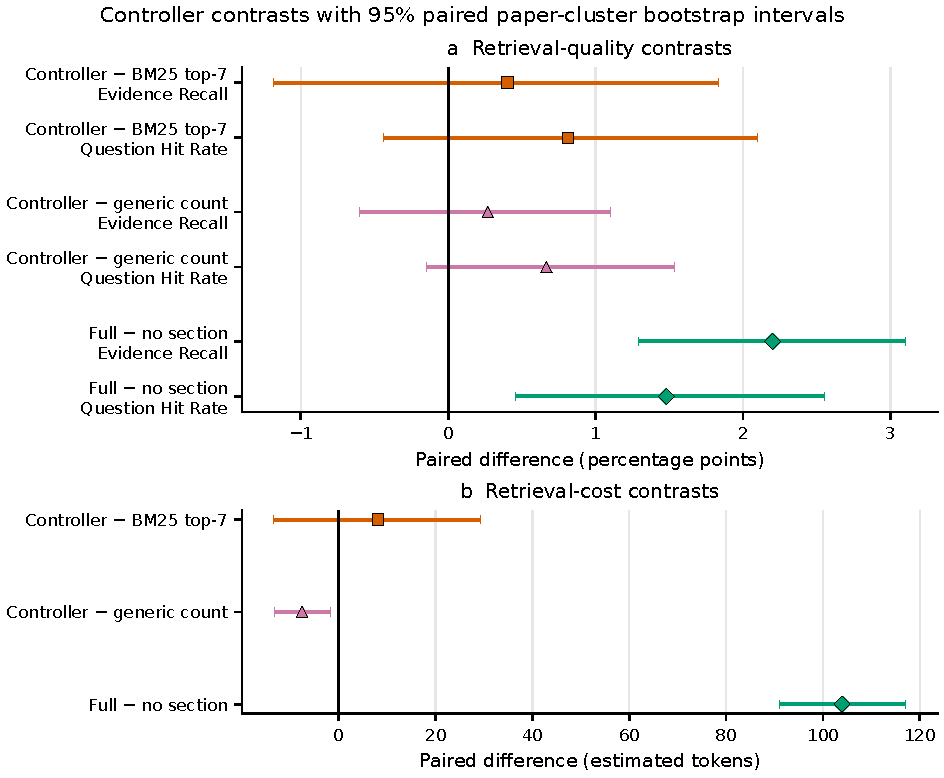
\includegraphics[width=0.94\textwidth]{figures/fig_paired_retrieval_effects.pdf}
\caption{Selected paired paper-level bootstrap differences. Points are observed differences and bars are 95\% percentile intervals over 5,000 paper-cluster replicates.}
\label{fig:paired-effects}
\end{figure}

\section{Section ablation and budget-matched controls}

The no-section ablation obtains 0.6879 recall and 0.8558 hit rate at 1,534 estimated tokens. Adding the section-aware definition and data branches increases recall by 0.0220 [0.0129, 0.0310], hit rate by 0.0148 [0.0046, 0.0255], and Average Best Overlap by 0.0167 [0.0109, 0.0225]. It also adds 104.0 estimated tokens [91.1, 117.1] and reduces Recall per 1,000 tokens by 0.0150. The full-versus-ablation result therefore shows that the complete policy buys additional coverage; it does not yet establish that section targeting is responsible.

\Cref{tab:mechanism} provides the necessary matched-budget comparison. AbstractOnly covers just 0.1063 of gold spans, while ReadAll reaches 0.9973 recall and a hit rate of 1.0 at an average estimated cost of 5,130 tokens. The two generic controls closely match ControllerV3's unit or token budget and obtain recall between 0.7064 and 0.7072.

\begin{table}[tb]
\centering
\caption{Supplementary retrieval controls on the complete QASPER test split.}
\label{tab:mechanism}
\small
\begin{tabular}{@{}lrrrrr@{}}
\toprule
Method & Recall & Hit rate & Avg. units & Est. tokens & Recall/1k \\
\midrule
AbstractOnly & 0.1063 & 0.2078 & 1.00 & 178 & 0.5972 \\
ReadAll & 0.9973 & 1.0000 & 29.43 & 5,130 & 0.1944 \\
GenericCountMatched & 0.7072 & 0.8639 & 7.76 & 1,645 & 0.4299 \\
GenericTokenMatched & 0.7064 & 0.8654 & 7.75 & 1,637 & 0.4315 \\
ControllerV3 & 0.7099 & 0.8706 & 7.76 & 1,638 & 0.4334 \\
\bottomrule
\end{tabular}
\end{table}

Against GenericCountMatched, ControllerV3 changes recall by 0.0027 with a 95\% paired interval of $[-0.0060,0.0110]$, and hit rate by 0.0067 $[-0.0015,0.0153]$. Against GenericTokenMatched, the recall difference is 0.0035 $[-0.0051,0.0118]$. These intervals do not show a clear independent aggregate benefit from section targeting. Taken together with the ablation, the evidence indicates that the full controller's extra coverage is largely explained by its extra budget. This is a mechanism-level negative result, not evidence that paper structure can never help individual questions.

\section{Question-dependent budgets}

The controller selects a mean of 7.76 units, a median of 7, and a range from 4 to 12. Its estimated evidence cost ranges from approximately 424 to 3,267 tokens. Compared question by question with BM25 top-7, ControllerV3 uses fewer tokens for 379 questions (26.1\%), the same number for 429 (29.6\%), and more for 643 (44.3\%). The near-equality of the average costs therefore conceals substantial reallocation across individual questions.

\begin{figure}[tb]
\centering
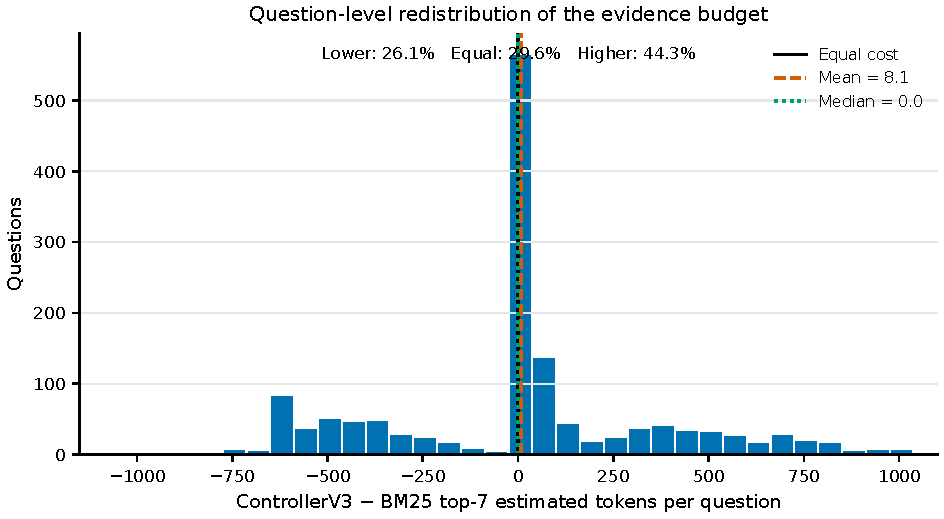
\includegraphics[width=0.92\textwidth]{figures/fig_controller_budget_distribution.pdf}
\caption{ControllerV3 budget distribution and its paired relationship to BM25 top-7.}
\label{fig:budget-distribution}
\end{figure}

The rule paths behave as intended. The 139 definition questions use a mean of 4.87 units and approximately 1,147 estimated tokens. The 643 result-or-data questions use 9.90 units and 1,897 tokens. Method-or-complex questions use 7.04 units and 1,665 tokens, while the default branch uses 5.02 units and 1,180 tokens. This is strong evidence that the policy allocates heterogeneous budgets. It is not evidence that the allocation is optimal, because a fixed top-7 achieves similar aggregate quality.

Action logs show that ReadTop3 and Stop occur for all 1,451 questions. Result/data expansion runs 643 times, table reading 604 times, method/complex expansion 427 times, and data-section expansion 351 times. Definition-introduction expansion runs 135 times; only four definition questions require the all-section fallback. Figure-caption expansion is rare, occurring for 18 questions and adding 27 units.

\section{Diagnostic error analysis}

At threshold 0.5, ControllerV3 hits evidence for 1,177 of the 1,352 questions with gold evidence. The diagnostic script classifies the remaining 175 cases. General controller-selection failures account for 96, data-evidence failures for 36, definition failures for 18, and cases where BM25 top-20 also misses or mapping is problematic for 18. The remainder consists of three figure failures, two missing-table failures, and two result-evidence failures.

One representative data failure asks, ``How big is the ANTISCAM dataset?'' The controller executes top-3, result/data expansion, data-section expansion, and table reading, selecting nine chunks and three table captions. Its best overlap is 0.3469, while BM25 top-20 contains a unit with overlap 1.0. The action type is plausible, but the configured caps do not reach the decisive evidence. This example illustrates a recurring limitation: coarse lexical question categories decide where to spend budget but do not rerank candidate units by answer sufficiency.

The categories are heuristic diagnostics, not human-adjudicated labels. Counts should therefore be read as engineering clues. They nevertheless identify two concrete improvements: stronger semantic ranking inside the candidate pool, and a learned or evidence-conditioned decision about whether an additional unit is likely to resolve the question.

\section{Supplementary answer generation}

All 608 unique prompts in the frozen sample complete successfully. There are no failed calls or length stops. The largest prompt contains 3,796 of the configured 8,192 context tokens, and the largest output contains 236 of the configured 256 output tokens. Prompt reuse avoids 196 calls, or 24.4\% of the 804 method--question records.

\begin{table}[tb]
\centering
\caption{Answer results on the frozen 201-question, 53-paper generation sample.}
\label{tab:generation}
\small
\begin{tabular}{@{}lrrrr@{}}
\toprule
Method & Answer F1 & EM & Prompt tokens & Output tokens \\
\midrule
BM25 top-7 & 0.3278 & 0.2040 & 1,992.46 & 11.55 \\
BM25 top-8 & 0.3468 & 0.2040 & 2,269.81 & 12.81 \\
ControllerV3 & 0.3280 & 0.2090 & 2,050.92 & 12.05 \\
ControllerV3 no section & 0.3137 & 0.1891 & 1,922.34 & 12.98 \\
\bottomrule
\end{tabular}
\end{table}

ControllerV3 and BM25 top-7 have almost identical F1 point estimates: 0.3280 and 0.3278. Their paired difference is 0.0002 with a 95\% interval of $[-0.0313,0.0312]$. The controller uses 58.5 more prompt tokens on average, with an interval of $[-1.8,115.2]$. Compared with top-8, its F1 is lower by 0.0188 $[-0.0502,0.0134]$ while using 218.9 fewer prompt tokens $[-284.7,-154.6]$. Compared with the no-section ablation, its F1 is higher by 0.0143 $[-0.0083,0.0385]$ and uses 128.6 more prompt tokens $[94.0,165.6]$. No answer-F1 comparison shows a clear sampled difference.

\begin{figure}[tb]
\centering
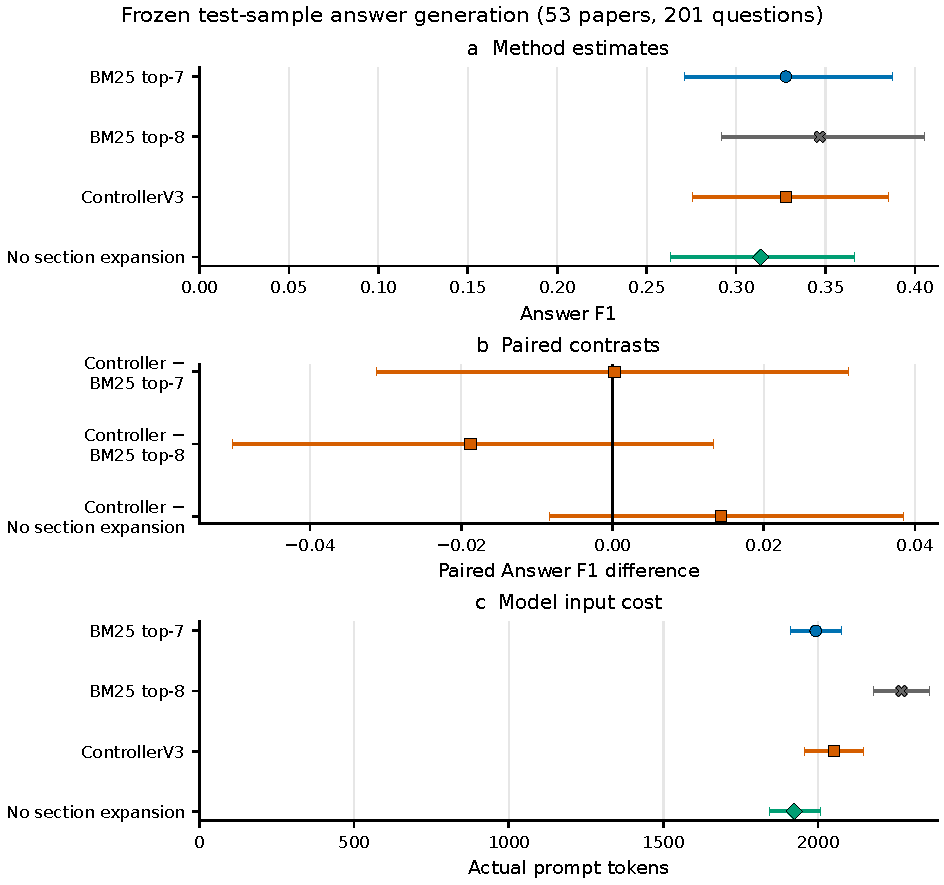
\includegraphics[width=0.94\textwidth]{figures/fig_generation_results.pdf}
\caption{Frozen generation-sample answer quality and actual prompt-token cost.}
\label{fig:generation-results}
\end{figure}

The generation sample supports a modest conclusion: ControllerV3 evidence is usable by the fixed local generator and yields sampled answer quality close to BM25 top-7. It does not demonstrate an answer-quality improvement, and its scope does not extend to the full test set or to larger generators.

